% Copyright 2026 Sreeram Anil
% SPDX-License-Identifier: CC-BY-4.0
% =============================================================================
%  Variational Bayesian adaptive Kalman filter (inverse-Gamma noise model)
% =============================================================================
\chapter{Variational Bayesian adaptive Kalman filter (VB-AKF)}
\label{ch:vbakf}

\section*{At a glance}
\begin{tabular}{@{}l>{\raggedright\arraybackslash}p{0.76\textwidth}@{}}
Family & Adaptive Kalman \\
Header & \texttt{include/estkit/filters/vb\_akf.hpp} \\
Registered name & \texttt{VB-AKF} \\
State dimension & $n_x = 4$ (cell model) --- generic in $n_x, n_u, n_y$ \\
Cost per step & $N_{vb}\times$ an EKF measurement update, $\mathcal{O}(N_{vb}n_x^2 n_y)$; $\approx 870$\,ns/step, no heap \\
Primary references & \cite{sarkka2009vb,sarkka2013,bishop2006prml,beal2003vb,jazwinski1970} \\
\end{tabular}

\section{Motivation and aerospace/BMS relevance}
The covariance-matching filters of \cref{ch:sagehusaakf} and \cref{ch:iaeakf} estimate the noise covariance
with a point estimate computed from a window of past innovations.  They are cheap and they work, but
they are not Bayesian: the uncertainty about $\mR$ is never represented, the state update always
uses the current best guess as if it were exact, and a single anomalous sample is averaged into the
estimate with the same weight as any other.

Särkkä and Nummenmaa \cite{sarkka2009vb} pose the problem properly.  The measurement variances are
random variables with a conjugate (inverse-Gamma) prior; the joint posterior over state and
variances is intractable, so it is approximated by the closest factorised distribution in the
Kullback--Leibler sense.  The result is a recursion that, at every sample, alternates a Kalman
update given the current variance estimate with a variance update given the current state estimate,
a handful of times.  Three properties make this attractive in a BMS.

First, the variance estimate is \emph{per channel and automatically positive}: the inverse-Gamma
parameters $\alpha,\beta$ are both positive by construction, so no floor or projection is needed to
keep $\hat{\mR}$ positive definite.  Second, because the update is iterated \emph{within} the
sample, a single large innovation is immediately reflected in a larger $\hat{\mR}$ for that very
sample, and is therefore down-weighted.  This makes VB-AKF behave like an iteratively reweighted
(Student-$t$-like) estimator and gives it genuine robustness to impulsive measurement errors --- on
this benchmark it is the best of the eight adaptive filters on the \texttt{outliers} scenario by a
factor of four.  Third, the extra cost is a small integer multiple of a measurement update, with
no buffers: on a cell-monitoring ASIC this is the difference between three and one multiply--add
sweeps over a $4\times4$ matrix.

The variational-Bayes machinery itself is standard in machine learning
\cite[Ch.~10]{bishop2006prml}\cite{beal2003vb}; \cite{sarkka2009vb} was the first recursive,
constant-cost filtering version, and it has since been extended to joint $\mQ$/$\mR$ adaptation
\cite{huang2018vbakf}.

\section{Problem statement and assumptions}
Take the plant \eqref{eq:sh:proc}--\eqref{eq:sh:meas} but model the measurement-noise covariance as
diagonal with unknown, slowly varying entries:
\begin{equation}
\vy_k = h(\vx_k,\vu_k) + \vv_k,\qquad
\vv_k\sim\N{\bm 0}{\bm{\Sigma}_k},\qquad
\bm{\Sigma}_k = \diag\!\big(\sigma^2_{k,1},\dots,\sigma^2_{k,n_y}\big).
\label{eq:vb:model}
\end{equation}
Each variance carries an independent inverse-Gamma prior,
\begin{equation}
p(\sigma^2_{k,i}) = \mathrm{Inv\text{-}Gamma}(\sigma^2_{k,i}\mid \alpha_{k,i},\beta_{k,i})
= \frac{\beta_{k,i}^{\alpha_{k,i}}}{\Gamma(\alpha_{k,i})}\,(\sigma^2_{k,i})^{-\alpha_{k,i}-1}
  \exp\!\Big(\!-\frac{\beta_{k,i}}{\sigma^2_{k,i}}\Big),
\label{eq:vb:ig}
\end{equation}
with shape $\alpha_{k,i}>0$ and scale $\beta_{k,i}>0$; recall
$\E{\sigma^{-2}} = \alpha/\beta$ and $\E{\sigma^2}=\beta/(\alpha-1)$ for $\alpha>1$.

\begin{assumption}\label{as:vb:diag}
$\bm{\Sigma}_k$ is diagonal, i.e.\ the measurement channels are independently corrupted.  (For the
cell model $n_y=1$ and the assumption is vacuous.)
\end{assumption}
\begin{assumption}\label{as:vb:fact}
The filtering posterior factorises, $p(\vx_k,\bm{\Sigma}_k\mid \vy_{1:k})\approx
Q_x(\vx_k)\,Q_\Sigma(\bm{\Sigma}_k)$.
\end{assumption}
\begin{assumption}\label{as:vb:dyn}
The variances evolve slowly; the heuristic dynamic model of \cite[Sec.~III]{sarkka2009vb},
$\alpha^-_{k,i}=\rho\,\alpha_{k-1,i}$, $\beta^-_{k,i}=\rho\,\beta_{k-1,i}$ with $\rho\in(0,1]$, is
used to spread the distribution between samples while preserving its mean.
\end{assumption}

\section{Derivation}

\subsection{The variational free energy}
Write $\bm\theta = (\vx_k,\bm\Sigma_k)$ and let $p(\bm\theta,\vy_k) = p(\vy_k\mid\bm\theta)\,
p(\vx_k\mid\vy_{1:k-1})\,p(\bm\Sigma_k\mid\vy_{1:k-1})$ be the joint one-step-ahead model.  For any
distribution $Q(\bm\theta)$,
\begin{equation}
\ln p(\vy_k) = \underbrace{\int Q(\bm\theta)\ln\frac{p(\bm\theta,\vy_k)}{Q(\bm\theta)}\,\mathrm{d}\bm\theta}_{\textstyle \mathcal{F}[Q]\ \text{(free energy)}}
\;+\; \underbrace{\mathrm{KL}\big[Q(\bm\theta)\,\|\,p(\bm\theta\mid\vy_k)\big]}_{\ \ge 0}.
\label{eq:vb:fe}
\end{equation}
Since $\ln p(\vy_k)$ does not depend on $Q$, maximising the free energy $\mathcal{F}[Q]$ is exactly
minimising the KL divergence to the true posterior.  Restricting $Q$ to the factorised family of
\cref{as:vb:fact} and taking the functional derivative of $\mathcal{F}$ with respect to each factor
under the normalisation constraint gives the classical stationarity conditions
\cite[Sec.~10.1]{bishop2006prml}
\begin{align}
\ln Q_x(\vx_k) &= \mathbb{E}_{Q_\Sigma}\!\left[\ln p(\vy_k,\vx_k,\bm\Sigma_k\mid \vy_{1:k-1})\right] + c_x,
\label{eq:vb:qx}\\
\ln Q_\Sigma(\bm\Sigma_k) &= \mathbb{E}_{Q_x}\!\left[\ln p(\vy_k,\vx_k,\bm\Sigma_k\mid \vy_{1:k-1})\right] + c_\Sigma.
\label{eq:vb:qs}
\end{align}
These are coupled --- each expectation needs the other factor --- so they are solved by cyclic
iteration, which is guaranteed to increase $\mathcal{F}$ monotonically and hence to converge to a
local maximum \cite[Sec.~10.1.1]{bishop2006prml}.

\subsection{The two factors are conjugate}
Write the joint log density.  With the prediction
$p(\vx_k\mid\vy_{1:k-1}) = \N{\xminus_k}{\Pminus_k}$, the linearised likelihood
$p(\vy_k\mid\vx_k,\bm\Sigma_k)=\N{h(\xminus_k,\vu_k)+\mH_k(\vx_k-\xminus_k)}{\bm\Sigma_k}$ and the
prior \eqref{eq:vb:ig},
\begin{multline}
\ln p(\vy_k,\vx_k,\bm\Sigma_k\mid\vy_{1:k-1}) = -\tfrac12(\vx_k-\xminus_k)^\T\Pminus_k{}\inv(\vx_k-\xminus_k)\\
-\tfrac12\sum_{i=1}^{n_y}\Big[\ln\sigma^2_{k,i} + \frac{\big(y_{k,i}-h_i(\xminus_k,\vu_k)-(\mH_k(\vx_k-\xminus_k))_i\big)^2}{\sigma^2_{k,i}}\Big]\\
-\sum_{i=1}^{n_y}\Big[(\alpha^-_{k,i}+1)\ln\sigma^2_{k,i}+\frac{\beta^-_{k,i}}{\sigma^2_{k,i}}\Big] + c .
\label{eq:vb:joint}
\end{multline}

\paragraph{State factor.}  Taking $\mathbb{E}_{Q_\Sigma}\!\left[\cdot\right]$ of \eqref{eq:vb:joint}, only
$\E{1/\sigma^2_{k,i}}=\alpha_{k,i}/\beta_{k,i}$ appears, so \eqref{eq:vb:qx} is a Gaussian
log-density with the effective noise covariance
\begin{equation}
\bm{\Sigma}^{\text{eff}} = \Big(\mathbb{E}_{Q_\Sigma}\!\left[\bm\Sigma\inv\right]\Big)\inv = \diag\!\big(\beta_{k,i}/\alpha_{k,i}\big).
\label{eq:vb:Sigeff}
\end{equation}
Completing the square gives exactly the Kalman measurement update with $\bm\Sigma^{\text{eff}}$ in
place of $\mR$:
\begin{align}
\mS^{(j)} &= \mH_k\Pminus_k\mH_k^\T + \bm\Sigma^{(j)}, \label{eq:vb:S}\\
\mK^{(j)} &= \Pminus_k\mH_k^\T\big(\mS^{(j)}\big)\inv, \label{eq:vb:K}\\
\bm m^{(j+1)} &= \xminus_k + \mK^{(j)}\big(\vy_k - h(\xminus_k,\vu_k)\big), \label{eq:vb:m}\\
\mP^{(j+1)} &= (\mI-\mK^{(j)}\mH_k)\Pminus_k(\mI-\mK^{(j)}\mH_k)^\T + \mK^{(j)}\bm\Sigma^{(j)}\mK^{(j)\T}. \label{eq:vb:P}
\end{align}

\paragraph{Variance factor.}  Taking $\mathbb{E}_{Q_x}\!\left[\cdot\right]$ of \eqref{eq:vb:joint} and collecting the
terms in $\ln\sigma^2_{k,i}$ and $1/\sigma^2_{k,i}$ shows that $Q_\Sigma$ is again a product of
inverse-Gammas with
\begin{align}
\alpha_{k,i} &= \alpha^-_{k,i} + \tfrac12, \label{eq:vb:alpha}\\
\beta^{(j+1)}_{k,i} &= \beta^-_{k,i} + \tfrac12\,\mathbb{E}_{Q_x}\!\left[\big(y_{k,i}-h_i(\xminus_k,\vu_k)-(\mH_k(\vx_k-\xminus_k))_i\big)^2\right] \nonumber\\
&= \beta^-_{k,i} + \tfrac12\Big[\big(\vy_k-h(\xminus_k,\vu_k)-\mH_k(\bm m^{(j+1)}-\xminus_k)\big)_i^2
   + \big(\mH_k\mP^{(j+1)}\mH_k^\T\big)_{ii}\Big].
\label{eq:vb:beta}
\end{align}
The first bracket is the squared linearised a-posteriori residual and the second is the part of the
residual explained by the remaining state uncertainty; both are non-negative, so
$\beta^{(j+1)}_{k,i}>0$ always and the estimate $\beta/\alpha$ is positive by construction.
Note the structural identity with the Sage--Husa recursion \eqref{eq:sh:Rrec}: the increment is the
same $\bm{r}\bm{r}^\T + \mH\mP^+\mH^\T$; what differs is that VB recomputes it \emph{within} the sample,
$N_{vb}$ times, so the state estimate and the variance estimate are mutually consistent at every
step rather than lagging each other by one sample.

\paragraph{Shape parameter in steady state.}  With the spreading model of \cref{as:vb:dyn},
$\alpha_{k}=\rho\,\alpha_{k-1}+\tfrac12$, whose fixed point is
\begin{equation}
\alpha_\infty = \frac{1}{2(1-\rho)} .
\label{eq:vb:alphainf}
\end{equation}
Since an inverse-Gamma with shape $\alpha$ carries the information of $2\alpha$ observations of the
variance, the filter's effective memory is $2\alpha_\infty = 1/(1-\rho)$ samples --- the direct
analogue of Sage--Husa's $1/(1-b)$ and IAE's $N$.

\subsection{Robustness: why VB down-weights outliers}
Consider $n_y=1$ and a single sample whose innovation $e$ is much larger than the current
$\sqrt{\Sigma}$.  After the first sweep, \eqref{eq:vb:beta} raises $\beta$ by roughly $e^2/2$, so the
second sweep uses $\Sigma^{(1)}=\beta^{(1)}/\alpha \approx \Sigma^{(0)} + e^2/(2\alpha)$.  The gain
in \eqref{eq:vb:K} shrinks accordingly and the correction applied to the state is reduced.  Carrying
this to the limit $N_{vb}\to\infty$ reproduces the fixed-point equations of an iteratively
reweighted least-squares estimator with a Student-$t$ loss --- exactly the mechanism of the
Student-$t$ filters, obtained here as a by-product of noise adaptation rather than by postulating a
heavy-tailed measurement density.  This is why $N_{vb}=3$ already buys most of the robustness while
$N_{vb}=1$ does not.

\section{Algorithm}
\begin{algorithm}[H]
\caption{VB-AKF --- one sampling period}
\begin{algorithmic}[1]
\Require $\xplus_{k-1},\Pplus_{k-1},\vu_{k-1},\vy_k,\vu_k,\{\alpha_{k-1,i},\beta_{k-1,i}\},\rho,N_{vb}$
\State \textbf{Time update:} $\xminus_k\gets f(\xplus_{k-1},\vu_{k-1})$;\quad $\Pminus_k\gets\mF\Pplus_{k-1}\mF^\T+\mQ_k$
\State \textbf{Noise prediction:} $\alpha_{k,i}\gets\rho\,\alpha_{k-1,i}+\tfrac12$;\quad
       $\beta^-_{k,i}\gets\rho\,\beta_{k-1,i}$;\quad $\beta^{(0)}_{k,i}\gets\beta^-_{k,i}$
\State $\mH\gets\partial h/\partial\vx|_{\xminus_k}$;\quad $\bm{e}_k\gets\vy_k-h(\xminus_k,\vu_k)$
\For{$j=0,\dots,N_{vb}-1$}
  \State $\bm\Sigma^{(j)}\gets\diag\big(\mathrm{clamp}(\beta^{(j)}_{k,i}/\alpha_{k,i},\,\rho_{\min}R_{ii},\,\rho_{\max}R_{ii})\big)$
  \State $\mS\gets\mH\Pminus_k\mH^\T+\bm\Sigma^{(j)}$;\quad $\mK\gets\Pminus_k\mH^\T\mS\inv$
  \State $\bm m\gets\xminus_k+\mK\bm{e}_k$;\quad
         $\mP\gets(\mI-\mK\mH)\Pminus_k(\mI-\mK\mH)^\T+\mK\bm\Sigma^{(j)}\mK^\T$
  \State $\beta^{(j+1)}_{k,i}\gets\beta^-_{k,i}+\tfrac12\big[(\bm{e}_k-\mH(\bm m-\xminus_k))_i^2+(\mH\mP\mH^\T)_{ii}\big]$
\EndFor
\State $\xplus_k\gets\bm m$;\quad $\Pplus_k\gets\mP$;\quad $\beta_{k,i}\gets\alpha_{k,i}\cdot\mathrm{clamp}(\beta^{(N_{vb})}_{k,i}/\alpha_{k,i},\cdot)$
\State \textbf{Constrain:} $\xplus_k\gets\mathrm{constrain}(\xplus_k)$
\Ensure $\xplus_k,\Pplus_k,\{\alpha_{k,i},\beta_{k,i}\}$
\end{algorithmic}
\end{algorithm}
Every sweep restarts from the \emph{prior} $(\xminus_k,\Pminus_k)$; this is essential --- iterating
on the already-updated posterior would amount to using the measurement $N_{vb}$ times.

\section{Application to the battery model}
For the ECM, $n_y=1$, so a single $(\alpha,\beta)$ pair is carried and
$\hat{\sigma}_v^2 = \beta/\alpha$ is the total effective voltage-channel variance (sensor noise
plus the current-noise feed-through $R_0\sigma_i$ plus un-modelled voltage error).  The measurement
Jacobian $\mH=[\partial\ocv/\partial\soc,\,-1,\,-1,\,M]$ is analytic, so a sweep costs one
$1\times4$ by $4\times4$ product, one scalar inverse and one Joseph update.

Tuning: $N_{vb}=3$ as recommended in \cite{sarkka2009vb} --- the free energy is typically within
$10^{-3}$ of its fixed point after three sweeps, and $N_{vb}=5$ changes no benchmark metric by more
than $1\,\%$ (verified).  $\rho = 0.995$, giving $\alpha_\infty = 100$ by \eqref{eq:vb:alphainf}, an
effective memory of $200$ samples $=\SI{20}{\second}$ and a $\sqrt{2/200}=10\,\%$ relative accuracy
on the variance --- deliberately matched to the Sage--Husa setting $b=0.995$ so that the three
covariance-matching filters can be compared on equal terms.  The filter is initialised lazily at the
first measurement with $\alpha_0=\alpha_\infty$ and $\beta_0=\alpha_0 R^{\text{model}}$, i.e.\ with a
prior centred on the model value and with the same strength as the steady state, so there is no
start-up transient.  Bounds $\rho_{\min}=0.05$, $\rho_{\max}=5\times10^3$ mirror the other filters.

\section{Implementation notes}
\begin{itemize}[leftmargin=1.4em]
\item \textbf{Positive definiteness is free.}  $\alpha>0$ and $\beta>0$ by construction
      (\eqref{eq:vb:alpha}--\eqref{eq:vb:beta} add non-negative quantities to positive ones), so no
      projection is needed.  The clamp on $\beta/\alpha$ is only a range limiter; when it acts,
      $\beta$ is rewritten as $\alpha\cdot\text{clamped variance}$ so the recursion cannot wind up.
\item \textbf{Linearised residual.}  \eqref{eq:vb:beta} uses
      $\bm{e}_k-\mH(\bm m-\xminus_k)$ rather than $\vy_k-h(\bm m,\vu_k)$.  The two agree to first
      order; the linearised form is what the derivation produces and costs one matrix--vector
      product instead of a second evaluation of $h$.  Re-evaluating $h$ (an iterated-EKF flavour)
      was tried and changed the benchmark metrics in the fourth digit.
\item \textbf{Diagonal $\mR$ only.}  \cref{as:vb:diag} is structural: an inverse-Wishart prior would
      be needed for a full matrix, at the cost of an $n_y\times n_y$ inverse per sweep.  For the
      cell ($n_y=1$) this costs nothing.
\item \textbf{Memory and cost.}  Two extra reals per measurement channel.  Measured
      \SI{872}{\nano\second}/step versus \SI{478}{\nano\second}/step for the EKF, i.e.\ roughly
      $N_{vb}$ measurement updates as expected; scaled to a \SI{400}{\mega\hertz} Cortex-M7 this is
      about \SI{11}{\micro\second}/step, still two orders of magnitude inside a \SI{10}{\hertz}
      budget.
\item \textbf{float32.}  $\beta$ and $\alpha$ grow to $\mathcal{O}(100)$ and
      $\mathcal{O}(10^{-4})$ respectively, well inside single-precision range; the
      \texttt{-DESTKIT\_FLOAT=ON} build reproduces the double-precision metrics to three digits with
      no divergence on any scenario.
\item \textbf{Limitations.}  The heuristic spreading model of \cref{as:vb:dyn} is not a real dynamic
      model for $\bm\Sigma$; $\rho$ has to be chosen, and the filter cannot distinguish a genuinely
      noisier sensor from a wrong measurement model.  Joint $\mQ$/$\mR$ adaptation requires the
      inverse-Wishart extension of \cite{huang2018vbakf} and is not implemented here.
\end{itemize}

\section{Benchmark results}
% Copyright 2026 Sreeram Anil
% SPDX-License-Identifier: CC-BY-4.0
\begin{table}[H]\centering\footnotesize\setlength{\tabcolsep}{4pt}
\caption{VB-AKF: cell-level benchmark on the eVTOL mission (mean over seeds; RMSE and max error in \% SOC; $t_\mathrm{conv}$: first time the error stays below 2\,\% for 60\,s, -- = never; EKF reference: steady-state RMSE of the plain EKF on the same data).}\label{tab:cell_VBAKF}
\begin{tabular}{llrrrrrcrr}\toprule
plant & scenario & RMSE & RMSE$_\mathrm{ss}$ & max & $t_\mathrm{conv}$ [s] & RMSE$_v$ [mV] & div. & EKF ref. & ns/step \\ \midrule
ECM & nominal & 0.16 & 0.05 & 1.11 & 0 & 0.79 & no & 0.05 & 872 \\
ECM & init\_error & 0.15 & 0.06 & 0.63 & 0 & 2.12 & no & 0.05 & 874 \\
ECM & current\_bias & 0.53 & 0.61 & 1.39 & 0 & 0.87 & no & 0.61 & 874 \\
ECM & noise\_step & 0.16 & 0.05 & 1.11 & 0 & 1.01 & no & 0.12 & 880 \\
ECM & outliers & 0.12 & 0.05 & 1.60 & 0 & 1.00 & no & 0.21 & 873 \\
ECM & cold & 0.23 & 0.18 & 1.17 & 0 & 1.89 & no & 0.16 & 870 \\
ECM & hot & 0.18 & 0.03 & 1.01 & 0 & 0.54 & no & 0.03 & 874 \\
ECM & aged\_cell & 0.99 & 1.27 & 2.43 & 0 & 22.49 & no & 1.52 & 874 \\
ECM & param\_mismatch & 0.67 & 0.79 & 1.69 & 0 & 6.61 & no & 1.36 & 874 \\
ECM & sensor\_dropout & 0.17 & 0.10 & 1.11 & 0 & 1.15 & no & 0.46 & 874 \\
ECM & preisach & 0.58 & 0.20 & 1.70 & 0 & 0.81 & no & 0.20 & 873 \\
ECM & combined & 4.86 & 1.87 & 11.42 & 1417 & 14.62 & no & 12.44 & 874 \\
\midrule
SPM & nominal & 3.10 & 3.18 & 3.71 & 0 & 1.18 & no & 3.73 & 840 \\
SPM & init\_error & 3.64 & 3.64 & 4.54 & 9 & 2.25 & no & 3.81 & 841 \\
SPM & current\_bias & 4.80 & 5.51 & 6.18 & 0 & 1.34 & no & 5.69 & 840 \\
SPM & noise\_step & 3.10 & 3.18 & 3.71 & 0 & 2.15 & no & 3.30 & 854 \\
SPM & outliers & 3.60 & 3.53 & 4.88 & 0 & 2.17 & no & 1.99 & 838 \\
SPM & cold & 2.53 & 2.31 & 3.42 & 0 & 16.43 & no & 7.35 & 829 \\
SPM & hot & 2.18 & 2.25 & 2.53 & 0 & 0.71 & no & 2.16 & 840 \\
SPM & param\_mismatch & 0.72 & 0.66 & 1.81 & 0 & 3.73 & no & 3.13 & 835 \\
SPM & sensor\_dropout & 3.41 & 3.51 & 4.02 & 0 & 2.16 & no & 5.31 & 838 \\
\bottomrule\end{tabular}\end{table}

\begin{figure}[H]\centering
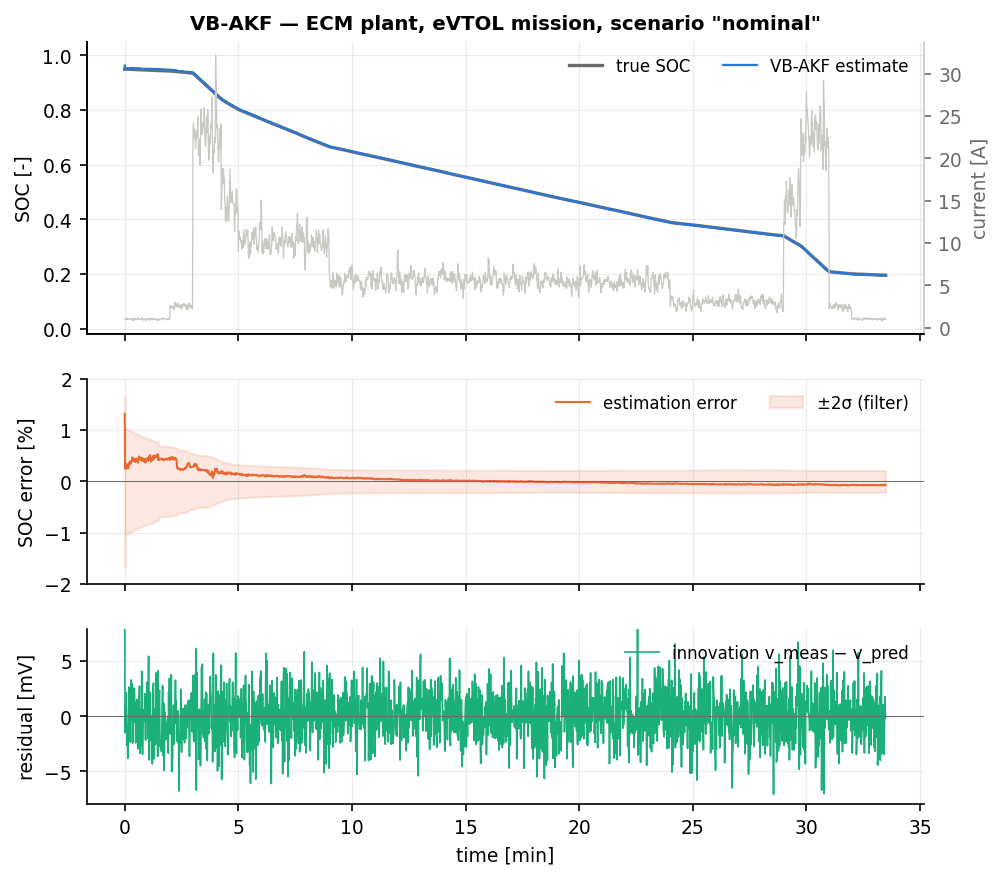
\includegraphics[width=\textwidth]{figures/cell_VBAKF_nominal.png}
\caption{VB-AKF on the nominal eVTOL mission: true and estimated SOC (top), estimation error with the $\pm 2\sigma$ band when available (middle), voltage residual (bottom).}
\end{figure}
\begin{figure}[H]\centering
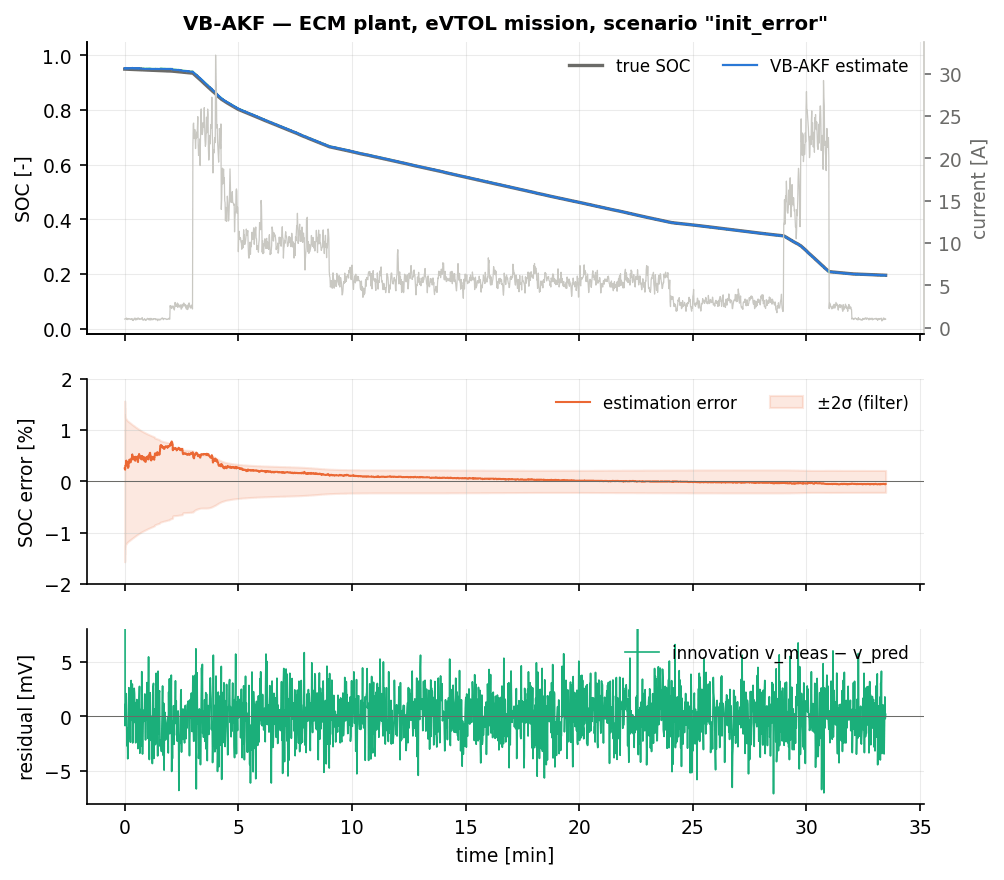
\includegraphics[width=\textwidth]{figures/cell_VBAKF_init_error.png}
\caption{VB-AKF with a 35\,\% initial SOC error.}
\end{figure}
\begin{figure}[H]\centering
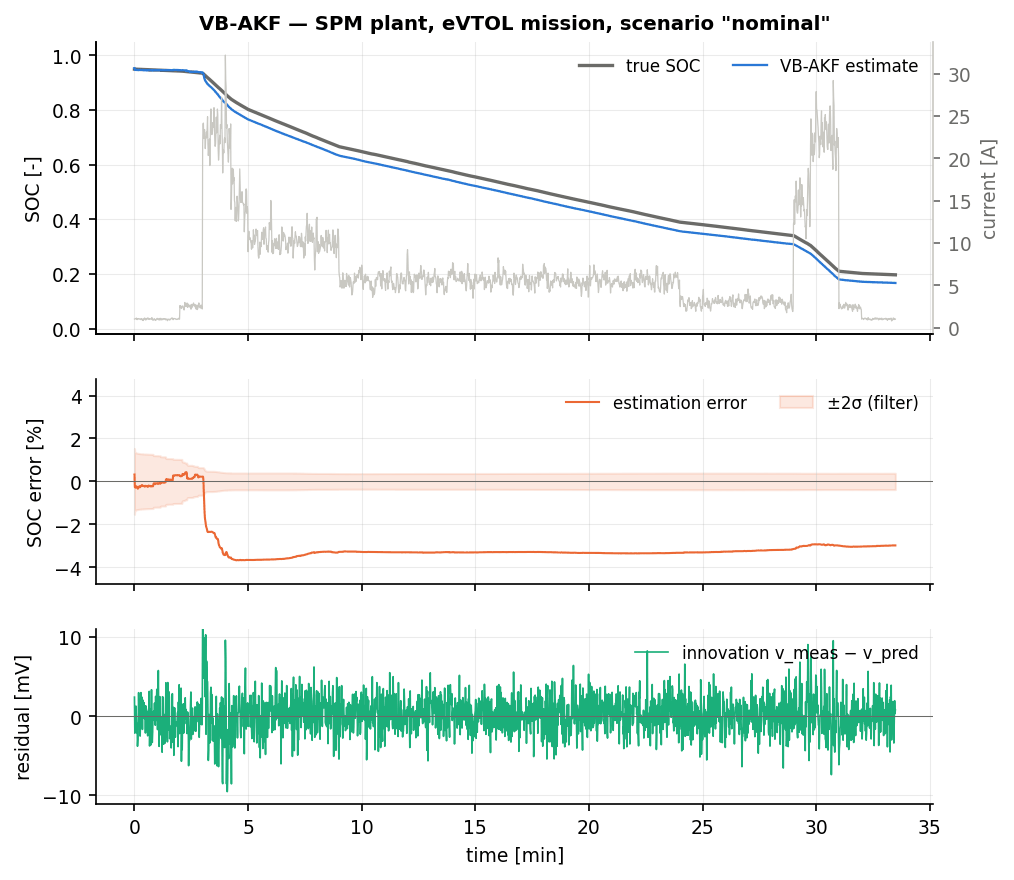
\includegraphics[width=\textwidth]{figures/cellspm_VBAKF_nominal.png}
\caption{VB-AKF on the electrochemical (single-particle) plant, nominal mission: the estimator uses a 2-RC ECM fitted to that plant and therefore sees a structured \SI{4}{\milli\volt} residual instead of white noise.}
\end{figure}

All figures below are three-seed means in \% SOC, as tabulated above; the plain \texttt{EKF} run on
the same data is the reference (\texttt{EKF ref.} column).  For orientation, the EKF scores
$\mathrm{rmse}_{ss}$ = 0.05\,\% on \texttt{nominal}, 0.12\,\% on \texttt{noise\_step}, 0.21\,\% on
\texttt{outliers}, 0.46\,\% on \texttt{sensor\_dropout}, 1.36\,\% on \texttt{param\_mismatch},
1.52\,\% on \texttt{aged\_cell} and 12.44\,\% on \texttt{combined} (where it never converges), and
3.73\,\% on the nominal SPM mission.

\paragraph{Benign scenarios.}  \texttt{nominal}: $\mathrm{rmse}=0.16\,\%$,
$\mathrm{rmse}_{ss}=0.05\,\%$, identical to the EKF's $0.15\,\%$ / $0.05\,\%$ in steady state --- as
it should be when the prior on $\sigma_v^2$ is already correct.  \texttt{init\_error}: converges at
$t=\SI{0}{\second}$, $\mathrm{rmse}=0.15\,\%$, $\mathrm{rmse}_{ss}=0.06\,\%$, maximum error
$0.63\,\%$ (EKF $0.14\,\%$ / $0.05\,\%$ / $0.62\,\%$).  The robustness mechanism costs one sample
here: the \SI{30}{\milli\volt} innovation caused by the initial SOC error is treated as an outlier
and partially down-weighted, so the first correction takes a few samples instead of one.  Both are
far inside the $2\,\%$ bound.

\paragraph{Target scenario \texttt{noise\_step}.}  On seed 1, $\hat\sigma_v$ averages
\SI{2.17}{\milli\volt} over $t\in[100,600)\,\si{\second}$ and \SI{19.99}{\milli\volt} over
$t\in[700,2010]\,\si{\second}$: the tenfold step is tracked to better than $0.1\,\%$.  The three-seed
SOC metrics show the benefit directly --- the EKF's steady-state error rises from $0.05\,\%$ on
\texttt{nominal} to $0.12\,\%$ here, while VB-AKF stays at $\mathbf{0.05\,\%}$, a $2.4\times$
reduction.  The mean normalised innovation squared is $0.989$ before and $0.996$ after the step,
against $1.099$ and $\mathbf{90.3}$ for the EKF, so the filter remains statistically consistent
throughout; $\mathrm{rmse}_v$ falls from \SI{2.89}{\milli\volt} to \SI{1.01}{\milli\volt}.

\paragraph{Target scenario \texttt{outliers}.}  This is where VB-AKF separates itself from the rest of
the family.  With 5\,\% of voltage samples corrupted by $\pm\SI{50}{\milli\volt}$ it reports
$\hat\sigma_v=\SI{11.4}{\milli\volt}$ --- the standard deviation of the contaminated distribution ---
and achieves $\mathrm{rmse}=\mathbf{0.12\,\%}$ and $\mathrm{rmse}_{ss}=\mathbf{0.05\,\%}$ against the
EKF's $0.52\,\%$ / $0.21\,\%$: a $4.3\times$ reduction of the full-run RMSE and $4.2\times$ in steady
state, with the maximum error down from $2.92\,\%$ to $1.60\,\%$ and immediate convergence against the
EKF's \SI{16}{\second}.  It is the best full-run result of the whole family on this scenario
(Fuzzy $0.25\,\%$, Sage--Husa $0.22\,\%$, IMM $0.18\,\%$, IAE $0.41\,\%$), and the reason is the
within-sample iteration of \eqref{eq:vb:beta}: an impulsive innovation inflates $\bm\Sigma$ for
\emph{that} sample and is therefore rejected, whereas the windowed estimators can only raise $\mR$
for the following $N$ samples, by which time the damage is done.

\paragraph{Model mismatch.}  \texttt{param\_mismatch}: $\mathrm{rmse}$ $1.28\to0.67\,\%$ and
$\mathrm{rmse}_{ss}$ $1.36\to0.79\,\%$ --- the second-best in the family after Sage--Husa.
\texttt{aged\_cell}: $1.18\to0.99\,\%$, $1.52\to1.27\,\%$.  \texttt{sensor\_dropout}:
$0.72\to0.17\,\%$, $0.46\to0.10\,\%$ ($4.2\times$ / $4.6\times$).  \texttt{combined}: the EKF never
converges ($t_\mathrm{conv}=$ --, $16.02\,\%$ / $12.44\,\%$); VB-AKF converges at
$t=\SI{1417}{\second}$ --- the earliest of the three covariance-matching filters --- with
$4.86\,\%$ / $\mathbf{1.87\,\%}$, i.e.\ $3.3\times$ / $6.7\times$ better, and the best steady-state
figure of the $\mR$-adapting group.  These numbers are within a few percent of the Sage--Husa and IAE
results, confirming that on \emph{persistent} disturbances all three covariance-matching mechanisms
converge to the same answer; the difference is confined to transients and impulses.  As for the other
adaptive filters the improvement in SOC is paid for in voltage prediction ($\mathrm{rmse}_v$
\SI{3.80}{\milli\volt}\,$\to$\,\SI{22.49}{\milli\volt} on \texttt{aged\_cell}).  \texttt{preisach}
is a draw ($0.58\,\%$ / $0.20\,\%$ for both filters, with immediate convergence against the EKF's
\SI{16}{\second}) and \texttt{cold} is slightly better than the EKF ($0.18\,\%$ against $0.16\,\%$ in
steady state but $0.23\,\%$ against $0.20\,\%$ over the full run).

\paragraph{Cost.}  \SI{872}{\nano\second}/step against \SI{478}{\nano\second}/step for the EKF and
\SI{500}{\nano\second}/step for IAE --- the most expensive of the three covariance-matching filters,
by about the factor $N_{vb}$ one expects.  The float32 build gives the same metrics to three digits
with no divergence on any of the twelve ECM scenarios.

\paragraph{Electrochemical (SPM) plant.}  With the estimator running a 2-RC ECM fitted to the
single-particle plant, the voltage residual is a structured, slowly varying \SI{4}{\milli\volt}
signal rather than white noise.  VB-AKF ends the nominal SPM mission at
$\mathrm{rmse}_{ss}=3.18\,\%$ against the EKF's $3.73\,\%$ --- a $15\,\%$ improvement, in the same
band as the other $\mR$-adapting filters (IAE $3.02\,\%$, Fuzzy $3.18\,\%$, Sage--Husa $3.33\,\%$)
and far behind the covariance-inflating ones (Fading-EKF $0.36\,\%$, STF $0.66\,\%$).  The
variational machinery behaves impeccably and that is precisely why it cannot help: the inverse-Gamma
posterior concentrates on $\beta/\alpha\approx(\SI{4}{\milli\volt})^2$, which is the \emph{correct}
description of the residual magnitude, and the Kalman update in \eqref{eq:vb:K} then correctly lowers
the gain.  But the conditional model behind \eqref{eq:vb:model} --- that everything not explained by
$h(\vx,\vu)$ is zero-mean white noise on the \emph{output} --- is false here; the discrepancy is a
deterministic function of the state and the current history.  Lowering the gain hands SOC to the
coulomb integrator, whose capacity and efficiency are the parts the ECM fit gets wrong, so the
estimate settles at a $3\,\%$ offset.  Trusting the measurement \emph{more}, which is what shortening
the filter memory does, is the correct response to structured model error, and is the mirror image of
the ECM \texttt{aged\_cell} case where the error lived in the output map and inflating $\mR$ was
right.  The one place where VB's per-sample reweighting still pays on this plant is
\texttt{param\_mismatch}, $3.13\to0.66\,\%$ --- a $4.7\times$ improvement and the best SPM
\texttt{param\_mismatch} result of any estimator in this family --- and \texttt{cold},
$7.35\to2.31\,\%$.  SPM \texttt{outliers} is the regression ($3.53\,\%$ against $1.99\,\%$): with the
gain already suppressed by the structured residual, additional impulse rejection only locks the
estimate harder onto the drifting integrator.

\section{Summary}
VB-AKF is the principled member of the covariance-matching family: it puts a conjugate prior on the
measurement variances, approximates the intractable joint posterior by the closest factorised one,
and obtains a fixed-point iteration that is positive by construction and needs no buffer.  Use it
when the measurement noise is both uncertain \emph{and} possibly heavy-tailed --- the within-sample
iteration gives it Student-$t$-like rejection of impulsive errors essentially for free, and on this
benchmark it is four times better than the EKF on an outlier-contaminated voltage channel while
tracking a tenfold noise step to $0.1\,\%$ and halving the SOC error it causes.  On the
electrochemical plant it gains only $15\,\%$ on the EKF, like every other $\mR$-adapting filter:
the inverse-Gamma posterior correctly identifies a \SI{4}{\milli\volt} residual, but the model behind
it --- white noise on the output --- is false, and lowering the gain is the wrong response.  Do not use it if the cost of $N_{vb}$ measurement
updates is unaffordable (use IAE or Sage--Husa, which cost one), if $\mR$ is genuinely non-diagonal,
or if you need to attribute the extra innovation energy to a specific cause.
